%%%%%%%%%%%%%%%%%%%%%%%%%%%%%%%%%%%%%%%%%%%%%%%%%%%%%%%%%%%%%%%%%%%%%%%%%%%%
%  第17回 例題11〜14（原本 20161215143926.pdf の p78/p79/p80/p81 より）
%  原本は「問題枠 →(指針)空欄→【KEY】」で解答が載っていないため，
%  【指針】と【解答】は本文の説明・練習問題の解答の解き方に合わせて書き起こした．
%  ・例題11 の指針は原本の【KEY】欄の下にある(5)への注意書きを含めてある．
%  ・例題12 だけは原本に(指針)・【KEY】の欄そのものが無い（本文の途中に置かれた
%    例題のため）。指針はこちらで補った．
%  ※ このファイルは記録用。実体は physics_ch17.tex に流し込み済み。
%%%%%%%%%%%%%%%%%%%%%%%%%%%%%%%%%%%%%%%%%%%%%%%%%%%%%%%%%%%%%%%%%%%%%%%%%%%%

%%%%%%%%%%%%%%%%%%%%  例題11（17.1 の直後）  %%%%%%%%%%%%%%%%%%%%
\begin{reidaiunit}
\begin{reidai}{等温変化}
\begin{zuright}{58mm}
\hspace{1zw}図のように一様な断面積を持つシリンダーに定積モル比熱が$C_V\U{J/mol\cdot K}$の理想気体を$n\U{mol}$封入した．ピストンは軽くて自由に動くことができ，棒が取り付けてある．最初，この気体の温度は$T_0\U{K}$，体積は$V_0\U{m^3}$であった．
\zusep
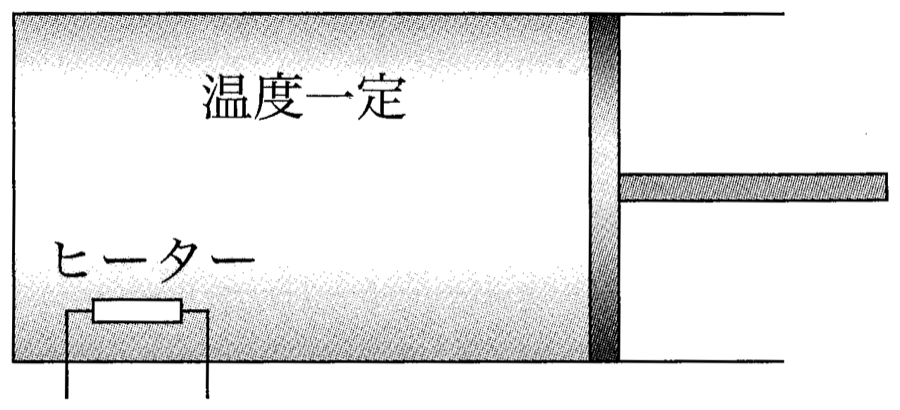
\includegraphics[keepaspectratio,width=58mm]{fig/ch17_ex11_cyl.png}
\end{zuright}
\hspace{1zw}シリンダー内にはヒーターが取り付けてあり，気体に対して熱を与えることができる．シリンダーおよびピストンは断熱材で出来ており，ヒーターによって与えた熱が大気に逃げることはないものとする．気体定数を$R\U{J/mol\cdot K}$として以下の問に答えよ．
\begin{komon}
\ko{1} 始めの状態における気体の圧力$P_0\U{Pa}$を求めよ．
\end{komon}
\hspace{1zw}ここで，気体が温度$T_0\U{K}$を保つようにピストンを操作しながら気体に熱をゆっくりと与え，体積を$V_1\U{m^3}$となるまで膨張させた．
\begin{komon}
\ko{2} 終状態における気体の圧力$P_1\U{Pa}$を求めよ．
\ko{3} 気体の体積が$V\U{m^3}$（$V_0<V<V_1$）のときの気体の圧力$P(V)\U{Pa}$を求めよ．
\ko{4} この状態変化を$P-V$図で表せ．
\ko{5} この変化において気体が外界に対してした仕事$w\U{J}$を求めよ．ただし，$\displaystyle\int\frac{1}{x}dx=\log|x|+C$（$C$は積分定数）である．
\ko{6} この変化における気体の内部エネルギーの増加量$\Delta U\U{J}$を求めよ．
\ko{7} ヒーターによって加えた熱量$Q\U{J}$を求めよ．
\end{komon}
\end{reidai}

\begin{sisinE}
温度が一定に保たれる状態変化を{\gtfamily 等温変化}という．等温変化では内部エネルギーが変化しないので，加えた熱はすべて気体が外界にする仕事になる．

(5) この状態変化では圧力$P$は一定ではないから，$w=P\Delta V$とは書けないことに注意せよ．体積が$V\U{m^3}$のときの圧力$P(V)$を求め，それを積分する．
\end{sisinE}

\Key{状態方程式 $PV=nRT$\quad 内部エネルギー変化 $\Delta U=nC_V\Delta T$\quad 気体のする仕事 $w=\displaystyle\int_{V_1}^{V_2}P\,dV$\quad 熱力学第一法則 $\Delta U=Q+(-w)$}

\begin{kaitou}
\begin{komon}
\ko{1} 始めの状態の状態方程式$P_0V_0=nRT_0$より，
       \Ana{P_0=\frac{nRT_0}{V_0}\U{Pa}\Ans}
\ko{2} 終状態でも温度は$T_0$のままであるから，状態方程式$P_1V_1=nRT_0$より，
       \Ana{P_1=\frac{nRT_0}{V_1}\U{Pa}\Ans}
\ko{3} 体積が$V$のときも温度は$T_0$であるから，状態方程式$P(V)\cdot V=nRT_0$より，
       \Ana{P(V)=\frac{nRT_0}{V}\U{Pa}\Ans}
\ko{4} (3)より$P-V$図は$PV=nRT_0$（一定）の双曲線の一部で，次図の通り．
       \begin{center}
       \ifbsAnaume
       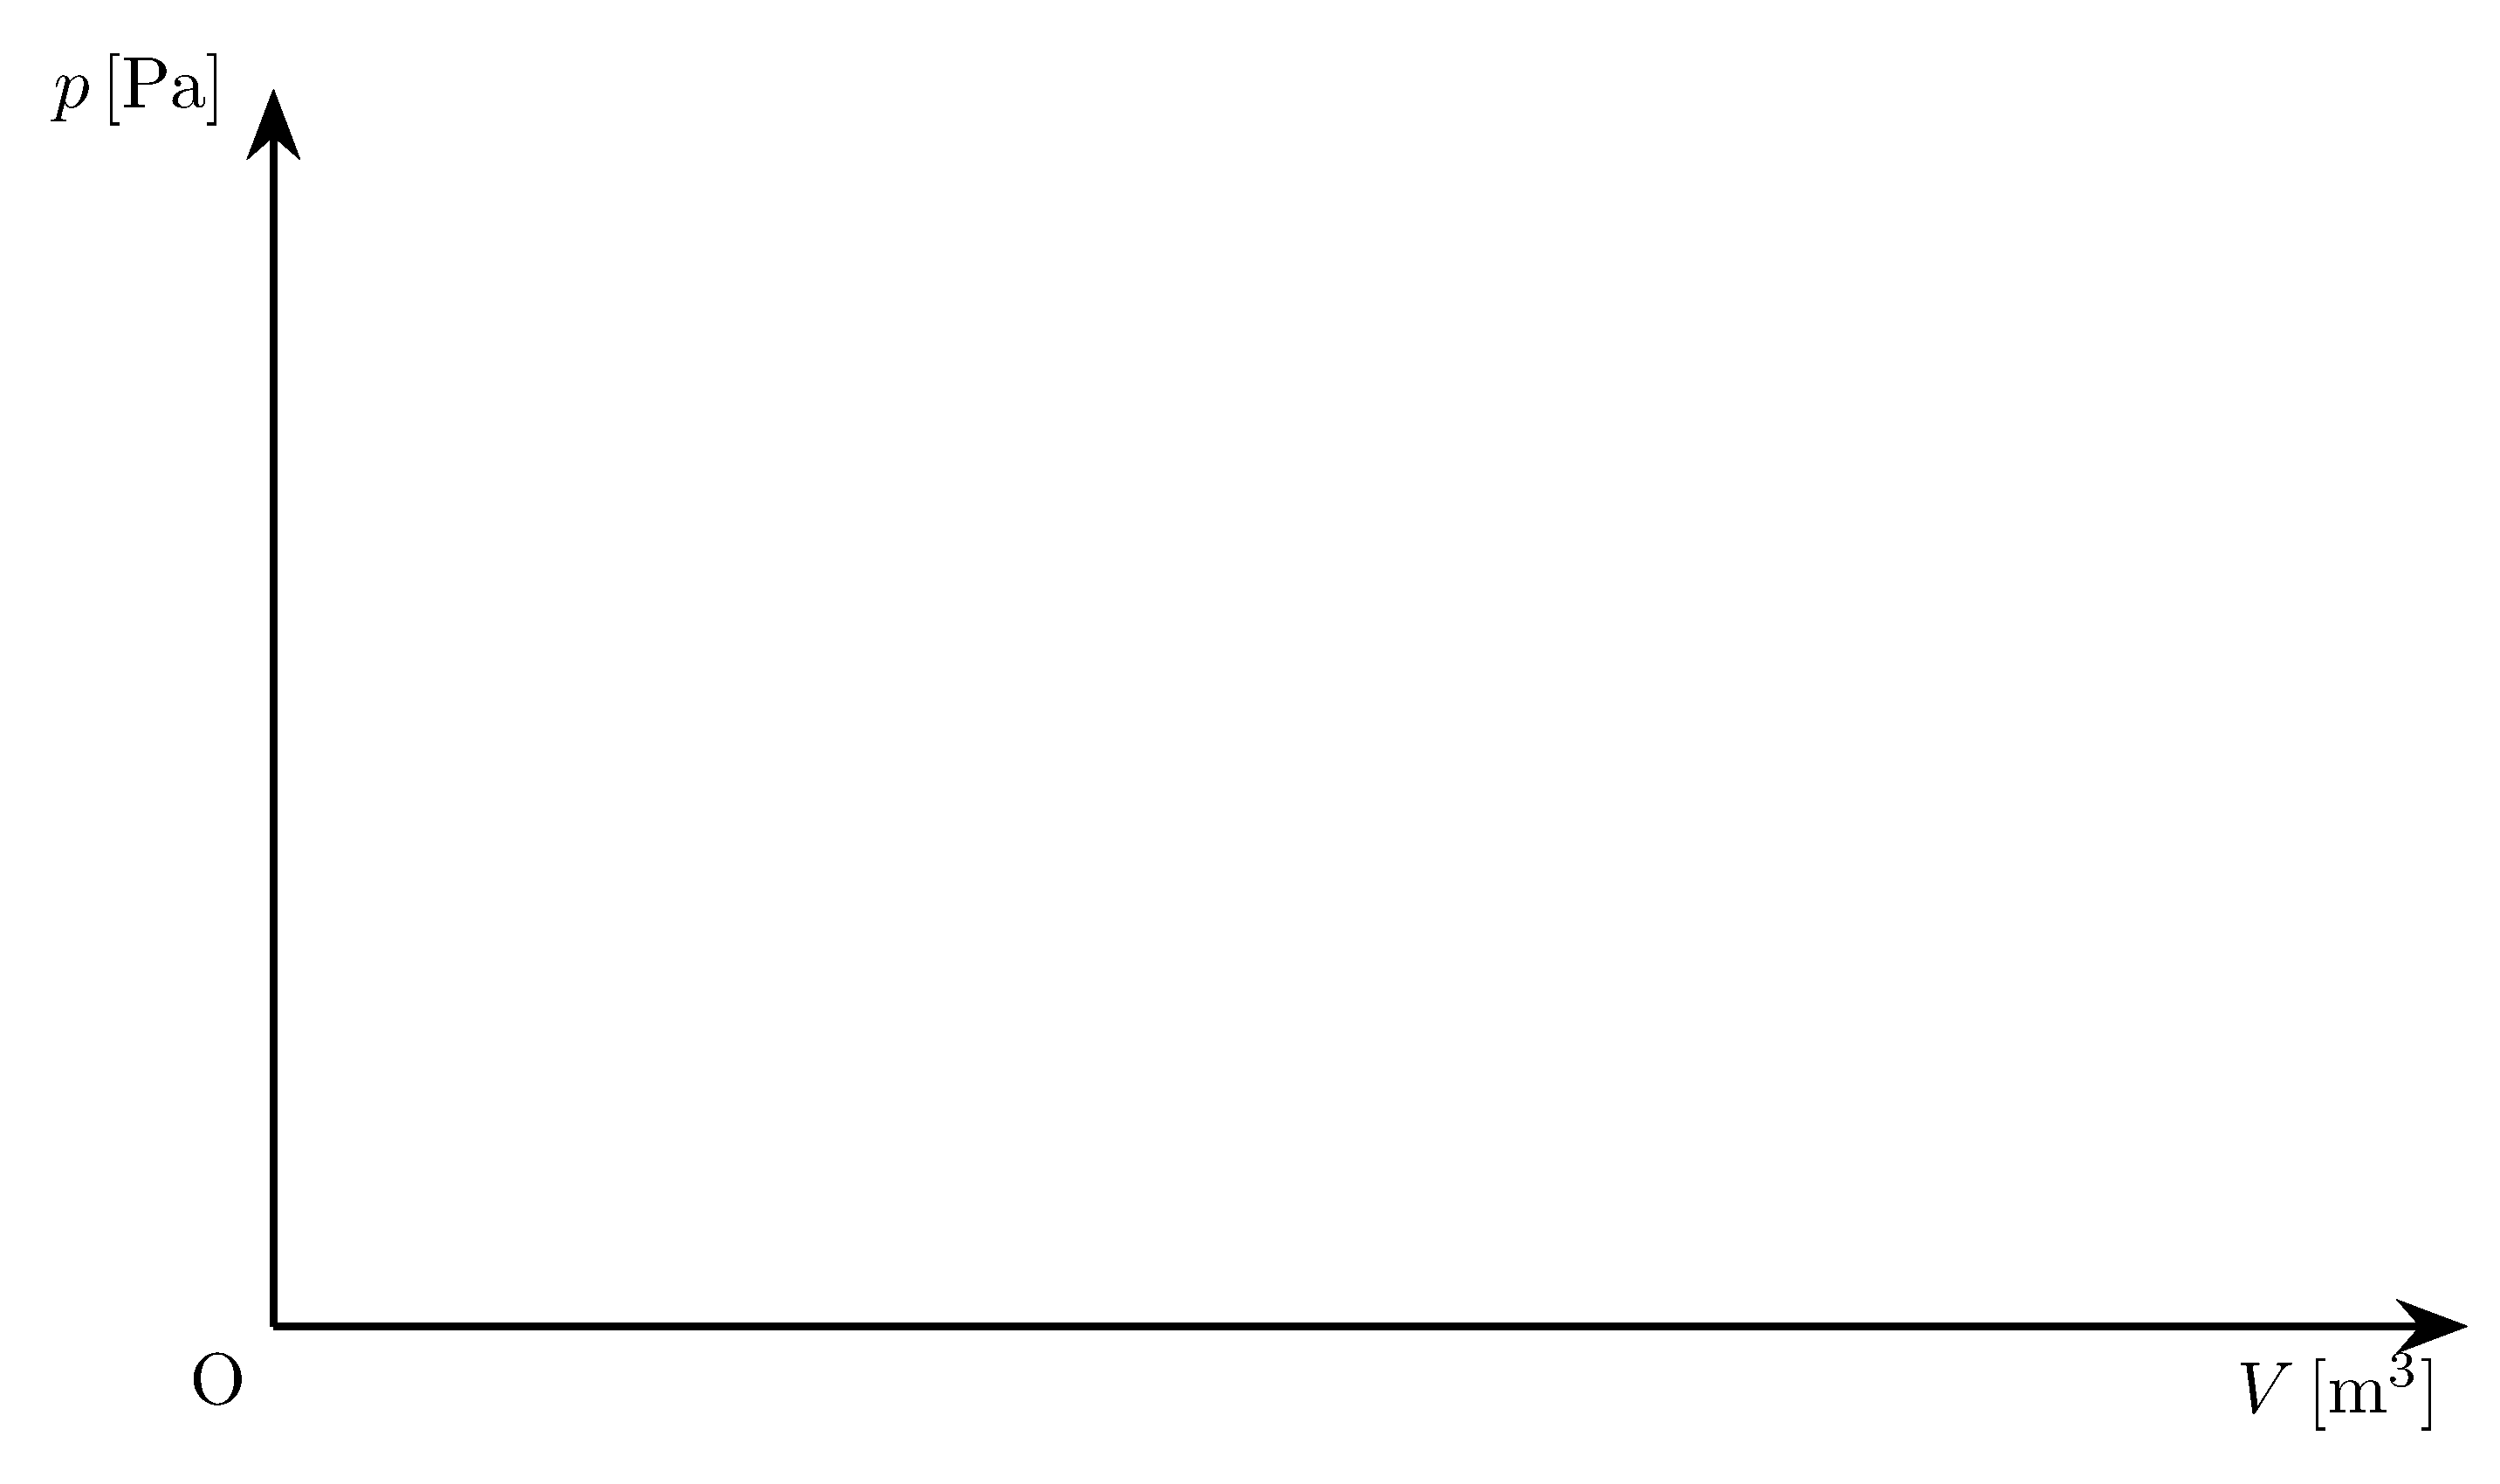
\includegraphics[keepaspectratio,width=96mm]{fig/ch17_ex11_pv_blank.png}
       \else
       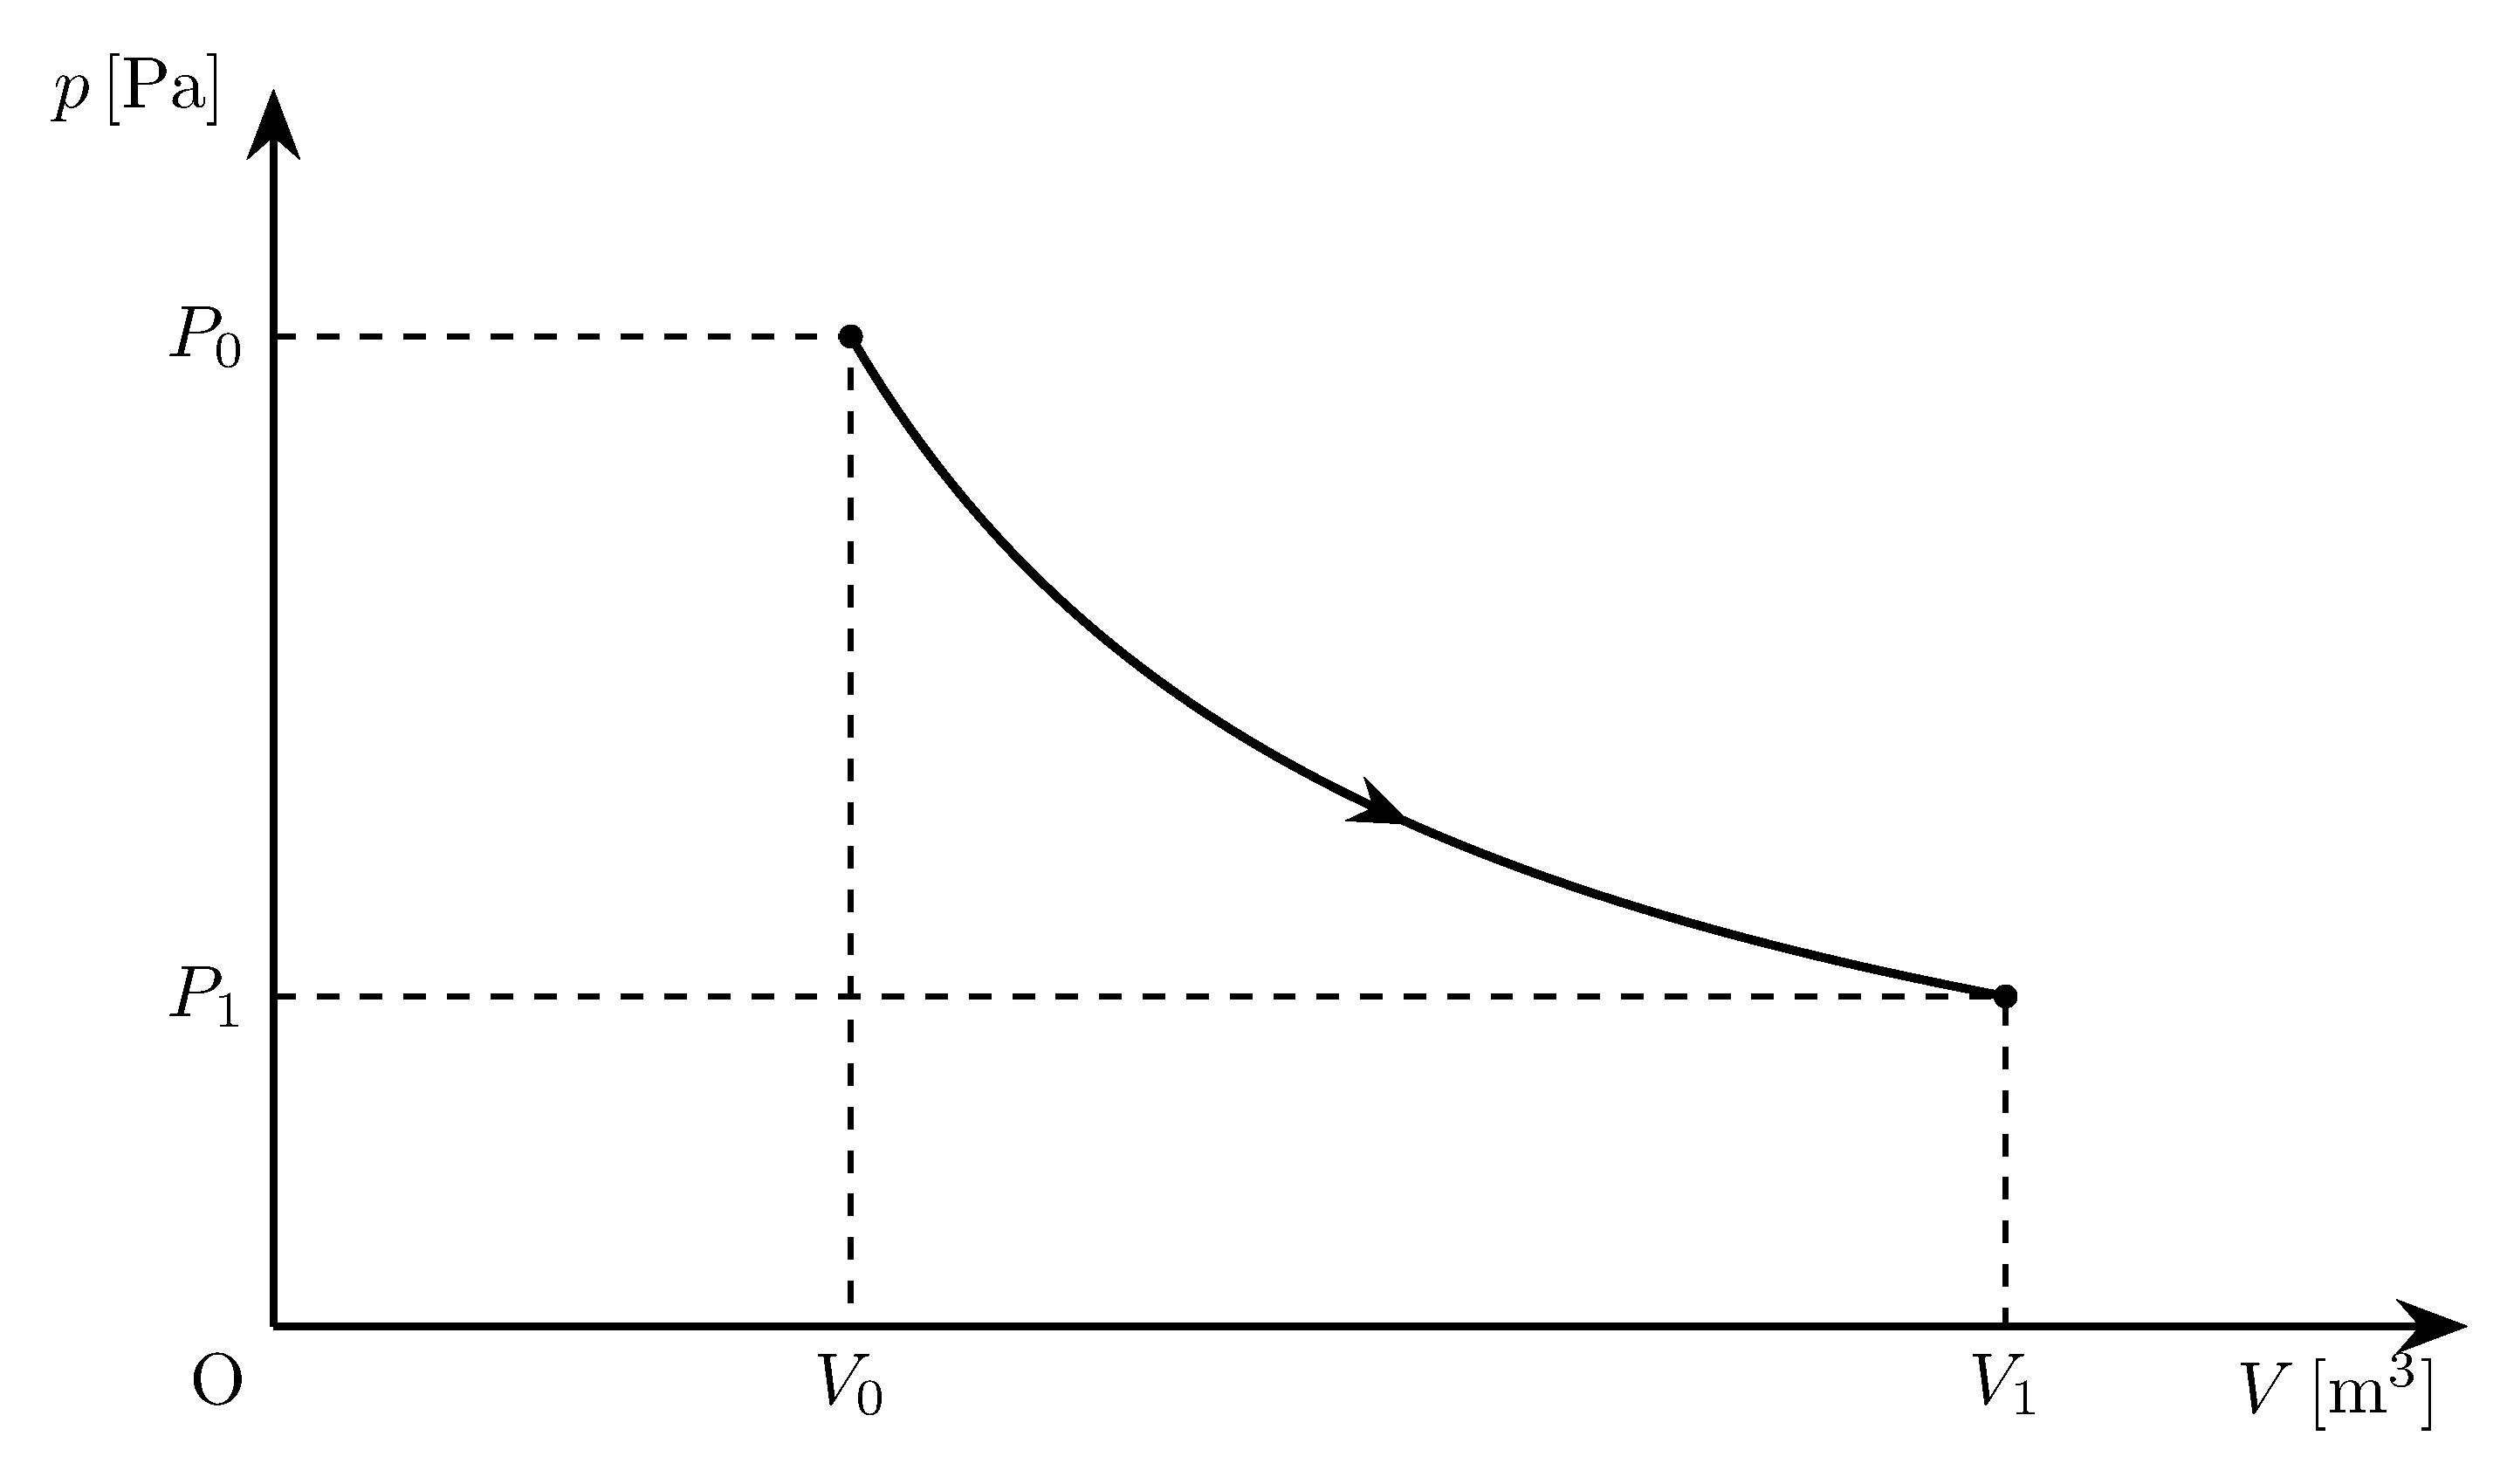
\includegraphics[keepaspectratio,width=96mm]{fig/ch17_ex11_pv.png}
       \fi
       \end{center}
       \hspace*{\fill}\Ans
\ko{5} $nRT_0$は定数であることに注意して，
       \Ana{w=\int_{V_0}^{V_1}P(V)dV=nRT_0\int_{V_0}^{V_1}\frac{1}{V}dV
             =nRT_0\log_e\frac{V_1}{V_0}\U{J}\Ans}
\ko{6} 温度が$T_0$のまま変化しないので$\Delta T=0$であり，
       \Ana{\Delta U=nC_V\Delta T=0\U{J}\Ans}
\ko{7} 熱力学第一法則$\Delta U=Q+(-w)$より，
       \Ana{Q=\Delta U+w=nRT_0\log_e\frac{V_1}{V_0}\U{J}\Ans}
       すなわち，加えた熱はすべて気体が外界にした仕事になっている．
\end{komon}
\end{kaitou}
\end{reidaiunit}

%%%%%%%%%%%%%%%%%%%%  例題12（17.2 の冒頭・ポアソンの法則の直前）  %%%%%%%%%%%%%%%%%%%%
\begin{reidaiunit}
\begin{reidai}{断熱変化}
\hspace{1zw}始状態において圧力$P_0\U{Pa}$，体積$V_0\U{m^3}$の理想気体を，外部との熱のやり取りを断ったまま体積が$V_1\U{m^3}$（ただし$V_1>V_0$）になるまで変化させる．終状態における気体の圧力を$P_1\U{Pa}$，気体定数を$R\U{J/mol\cdot K}$，気体の定積モル比熱を$C_V\U{J/mol\cdot K}$として以下の問に答えよ．
\begin{komon}
\ko{1} 内部エネルギー変化$\Delta U\U{J}$，気体が外にした仕事$w\U{J}$，吸熱量$Q\U{J}$を求めよ．
\ko{2} 膨張過程なので$w>0$である事を利用して，この変化によって気体の温度は増加するか，減少するか，答えよ．
\end{komon}
\end{reidai}

\begin{sisinE}
熱の出入りを断った状態変化なので$Q=0$である．与えられているのは$P$と$V$だけで温度が与えられていないが，状態方程式$PV=nRT$を使えば$nRT$を$PV$に置き換えられるので，$\Delta U=nC_V\Delta T$は$P$, $V$だけで表せる．
\end{sisinE}

\begin{kaitou}
\begin{komon}
\ko{1} 断熱変化であるから，
       \Ana{Q=0\U{J}\Ans}
       気体のモル数を$n\U{mol}$，始状態・終状態の温度を$T_0\U{K}$, $T_1\U{K}$とすると，状態方程式より$P_0V_0=nRT_0$, $P_1V_1=nRT_1$であるから，
       \Ana{\Delta U=nC_V(T_1-T_0)=\frac{C_V}{R}(P_1V_1-P_0V_0)\U{J}\Ans}
       熱力学第一法則$\Delta U=Q+(-w)$に$Q=0$を代入して，
       \Ana{w=-\Delta U=\frac{C_V}{R}(P_0V_0-P_1V_1)\U{J}\Ans}
\ko{2} (1)より$\Delta U=-w$であり，$w>0$であるから$\Delta U<0$である．$\Delta U=nC_V\Delta T$で$nC_V>0$であるから$\Delta T<0$，すなわち気体の温度は{\gtfamily 減少する}．\hspace*{\fill}\Ans
\end{komon}
\end{kaitou}
\end{reidaiunit}

%%%%%%%%%%%%%%%%%%%%  例題13（17.2 の末尾・等温曲線と断熱曲線の比較の直後）  %%%%%%%%%%%%%%%%%%%%
\begin{reidaiunit}
\begin{reidai}{ポアソンの式の利用}
\begin{zuright}{50mm}
\hspace{1zw}図のように一様な断面積を持つシリンダーに定積モル比熱が$C_V\U{J/mol\cdot K}$の理想気体を$n\U{mol}$封入した．ピストンは軽くて自由に動くことができ，外気圧とシリンダー内の気体の圧力とが常につり合いを保つ．シリンダーおよびピストンは断熱材で出来ており，外界との熱のやり取りはない．最初，この気体の温度は$T_0\U{K}$，体積は$V_0\U{m^3}$であり，ピストンは静止していた．
\zusep
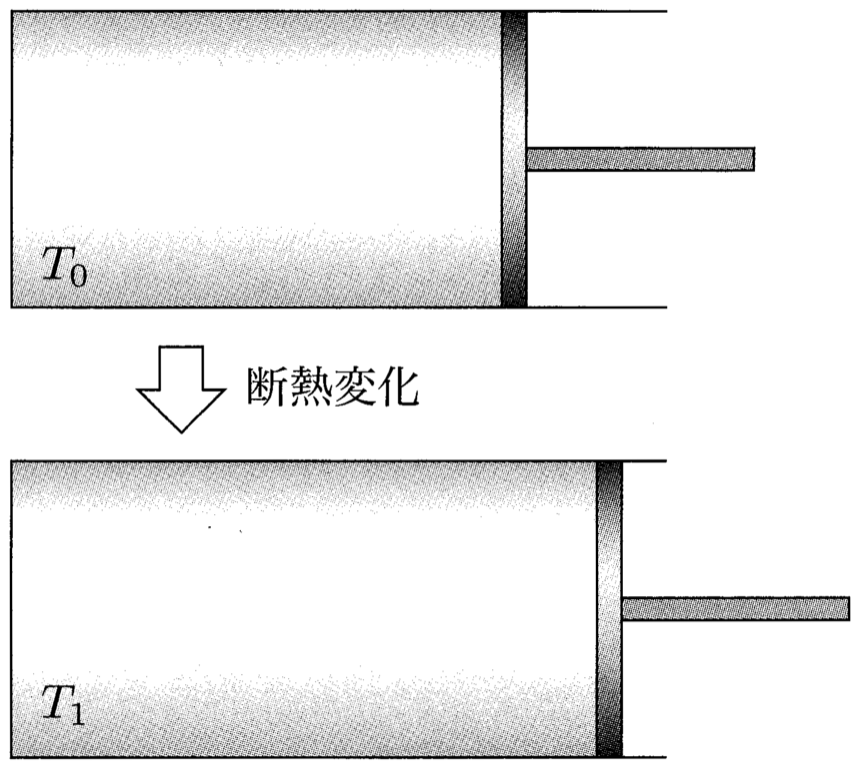
\includegraphics[keepaspectratio,width=50mm]{fig/ch17_ex13_cyl.png}
\end{zuright}
\hspace{1zw}この状態から外気圧をゆっくりと変化させ，気体の温度が$T_1\U{K}$($<T_0$)となるまで変化させた．理想気体が断熱変化するときは比熱比を$\gamma$として，ポアソンの式$PV^\gamma=（一定）$が成立することを用いてよい．気体定数を$R\U{J/mol\cdot K}$として以下の問に答えよ．
\begin{komon}
\ko{1} この状態変化を$P-V$図で表せ．ただし，終状態の体積を$V_1\U{m^3}$として図示せよ．
\ko{2} この気体が始状態から定温条件で体積$V_1\U{m^3}$となるまで変化した場合，気体はどのような曲線上を動くか．(1)の$P-V$図に点線で記入せよ．
\ko{3} この気体の内部エネルギー変化$\Delta U\U{J}$を求めよ．
\ko{4} この気体が外界にした仕事$w\U{J}$を求めよ．
\ko{5} 終状態における気体の体積$V_1\U{m^3}$を求めよ．
\end{komon}
\end{reidai}

\begin{sisinE}
温度が下がる断熱変化であるから，気体は外界に仕事をして膨張する（$V_1>V_0$）．$P-V$図では断熱曲線は等温曲線より急な右下がりの曲線になるので，同じ体積$V_1$まで変化させたとき断熱変化の方が圧力は低い．

断熱変化では$Q=0$なので，仕事$w$は積分せずとも熱力学第一法則$\Delta U=Q+(-w)$から求まる．体積を問われている(5)では，$P$と$V$を結ぶ$PV^\gamma=（一定）$ではなく$T$と$V$を結ぶ$TV^{\gamma-1}=（一定）$を使う．
\end{sisinE}

\Key{断熱変化中は比熱比$\gamma=\dfrac{C_P}{C_V}$を用いて $PV^\gamma=（一定）$, $TV^{\gamma-1}=（一定）$ が成立する}

\begin{kaitou}
\begin{komon}
\item[{\makebox[1.9zw][r]{(1)(2)}}] 断熱変化（実線）は$PV^\gamma=（一定）$，等温変化（点線）は$PV=（一定）$の曲線である．$\gamma>1$であるから断熱曲線の方が急になり，次図の通り．
       \begin{center}
       \ifbsAnaume
       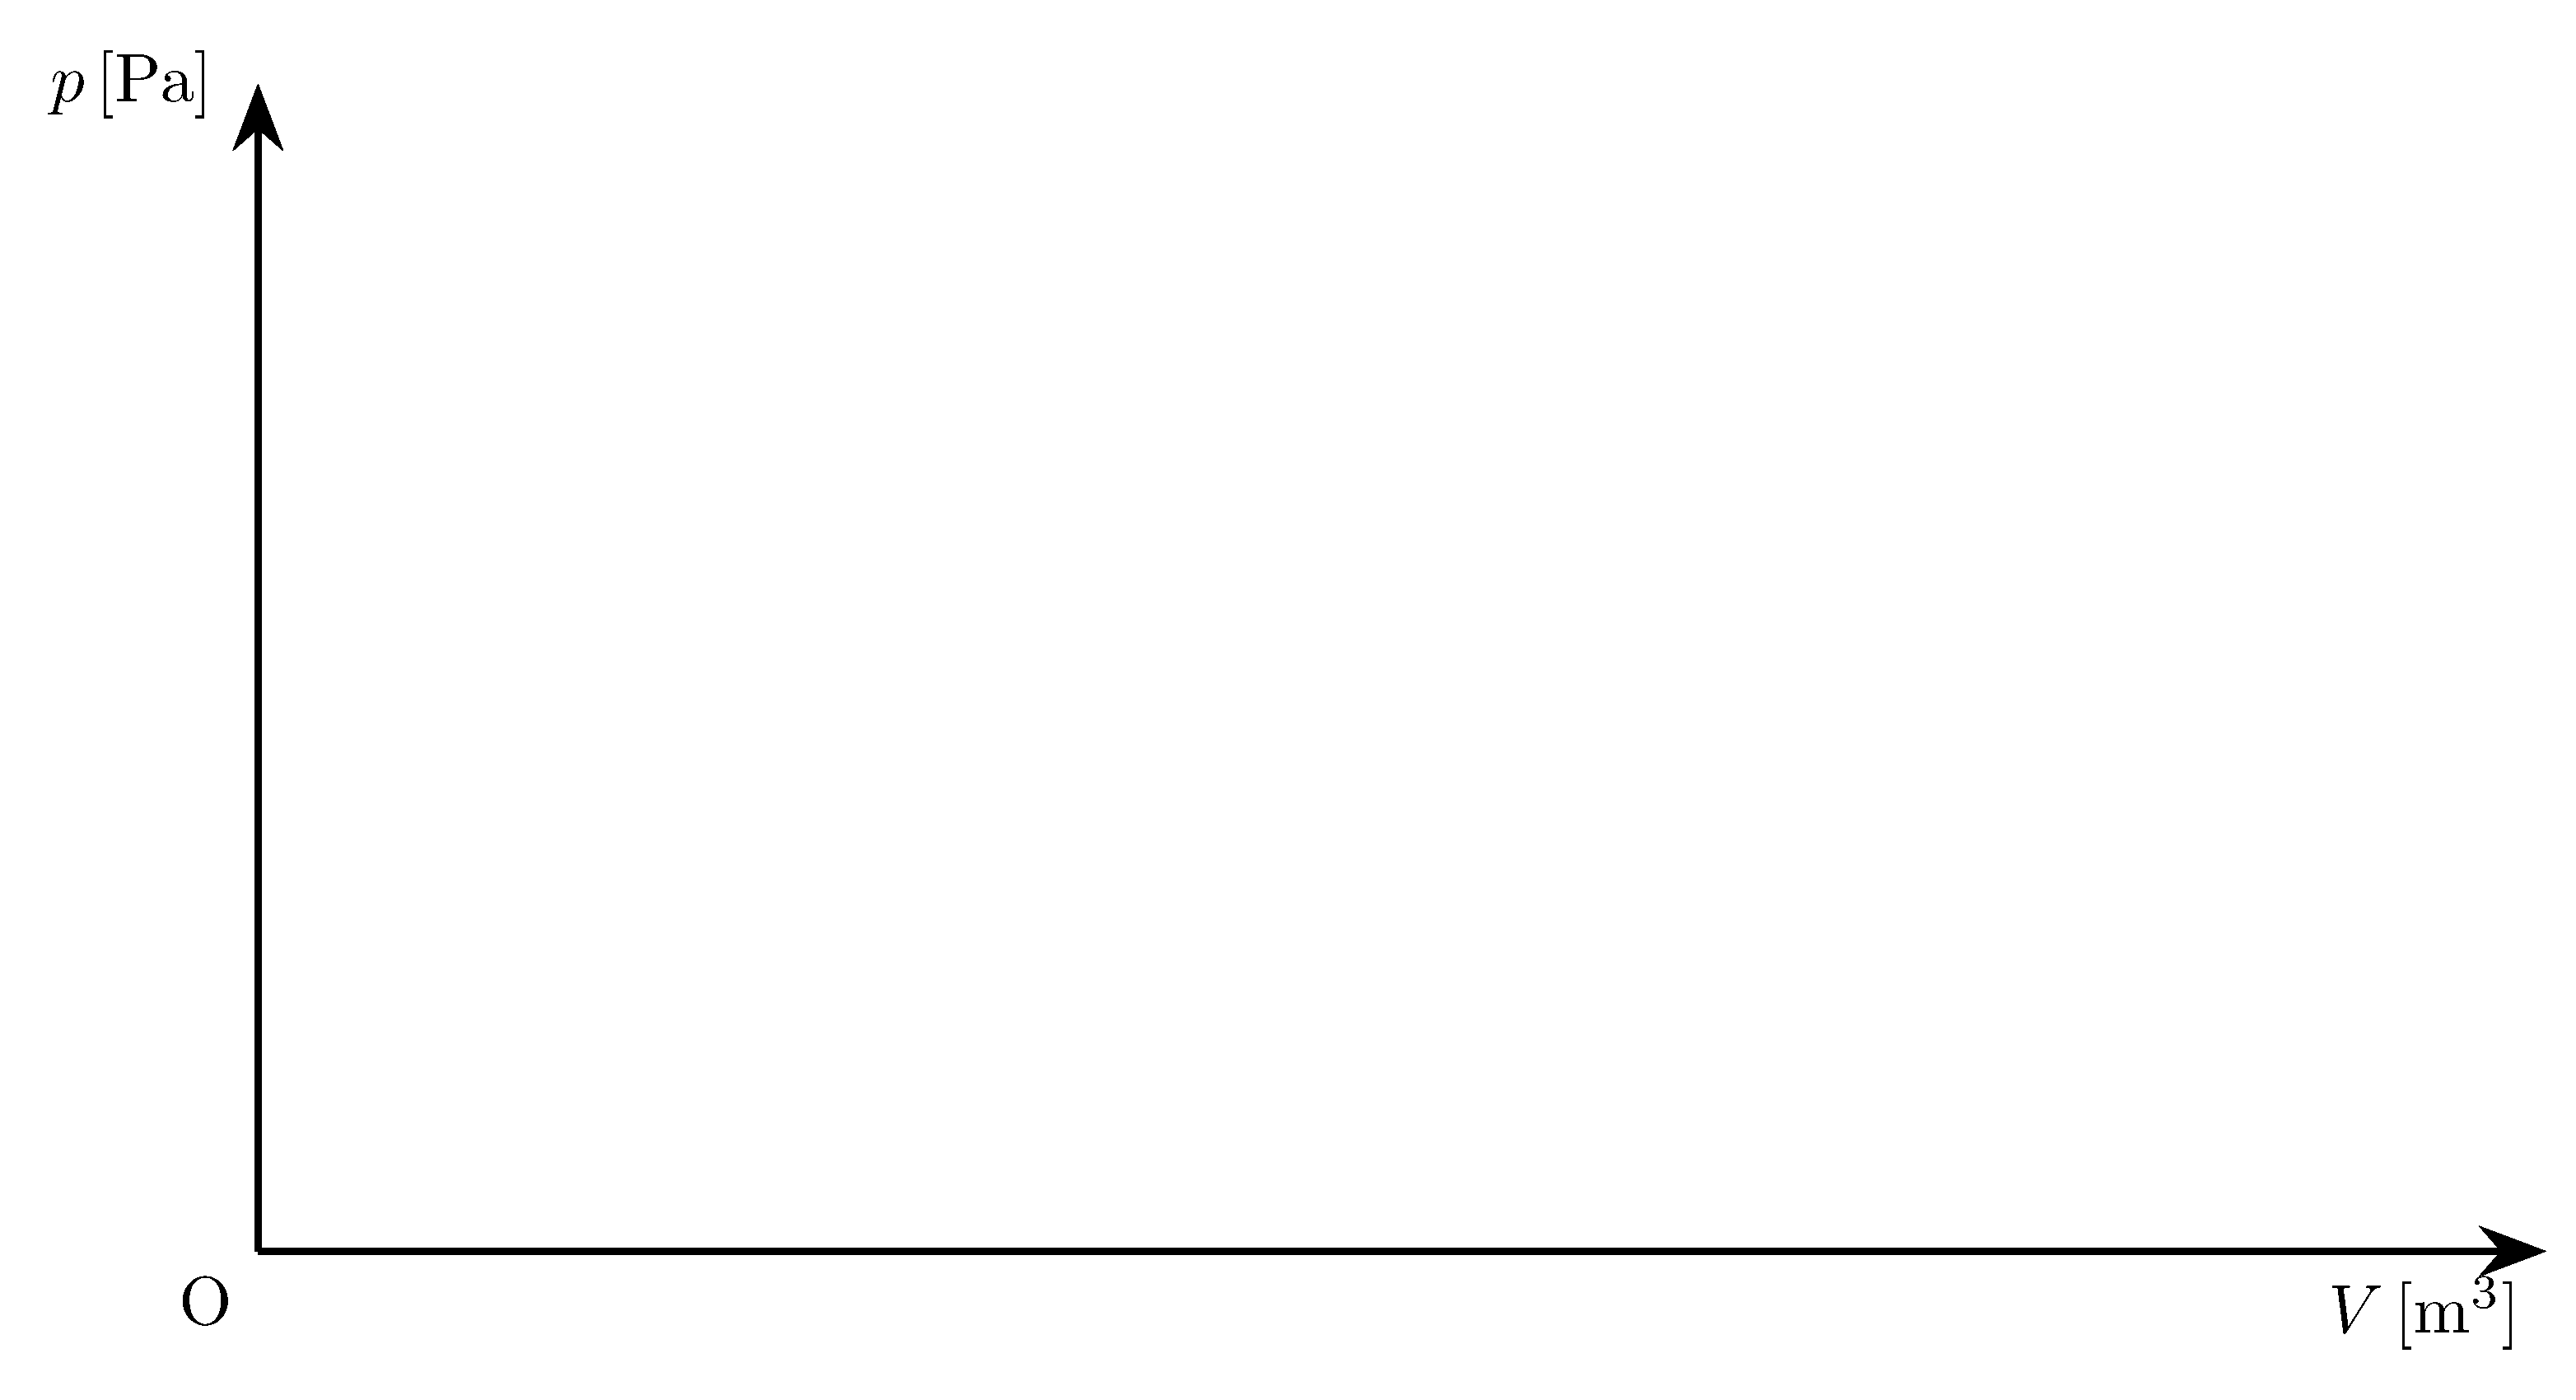
\includegraphics[keepaspectratio,width=106mm]{fig/ch17_ex13_pv_blank.png}
       \else
       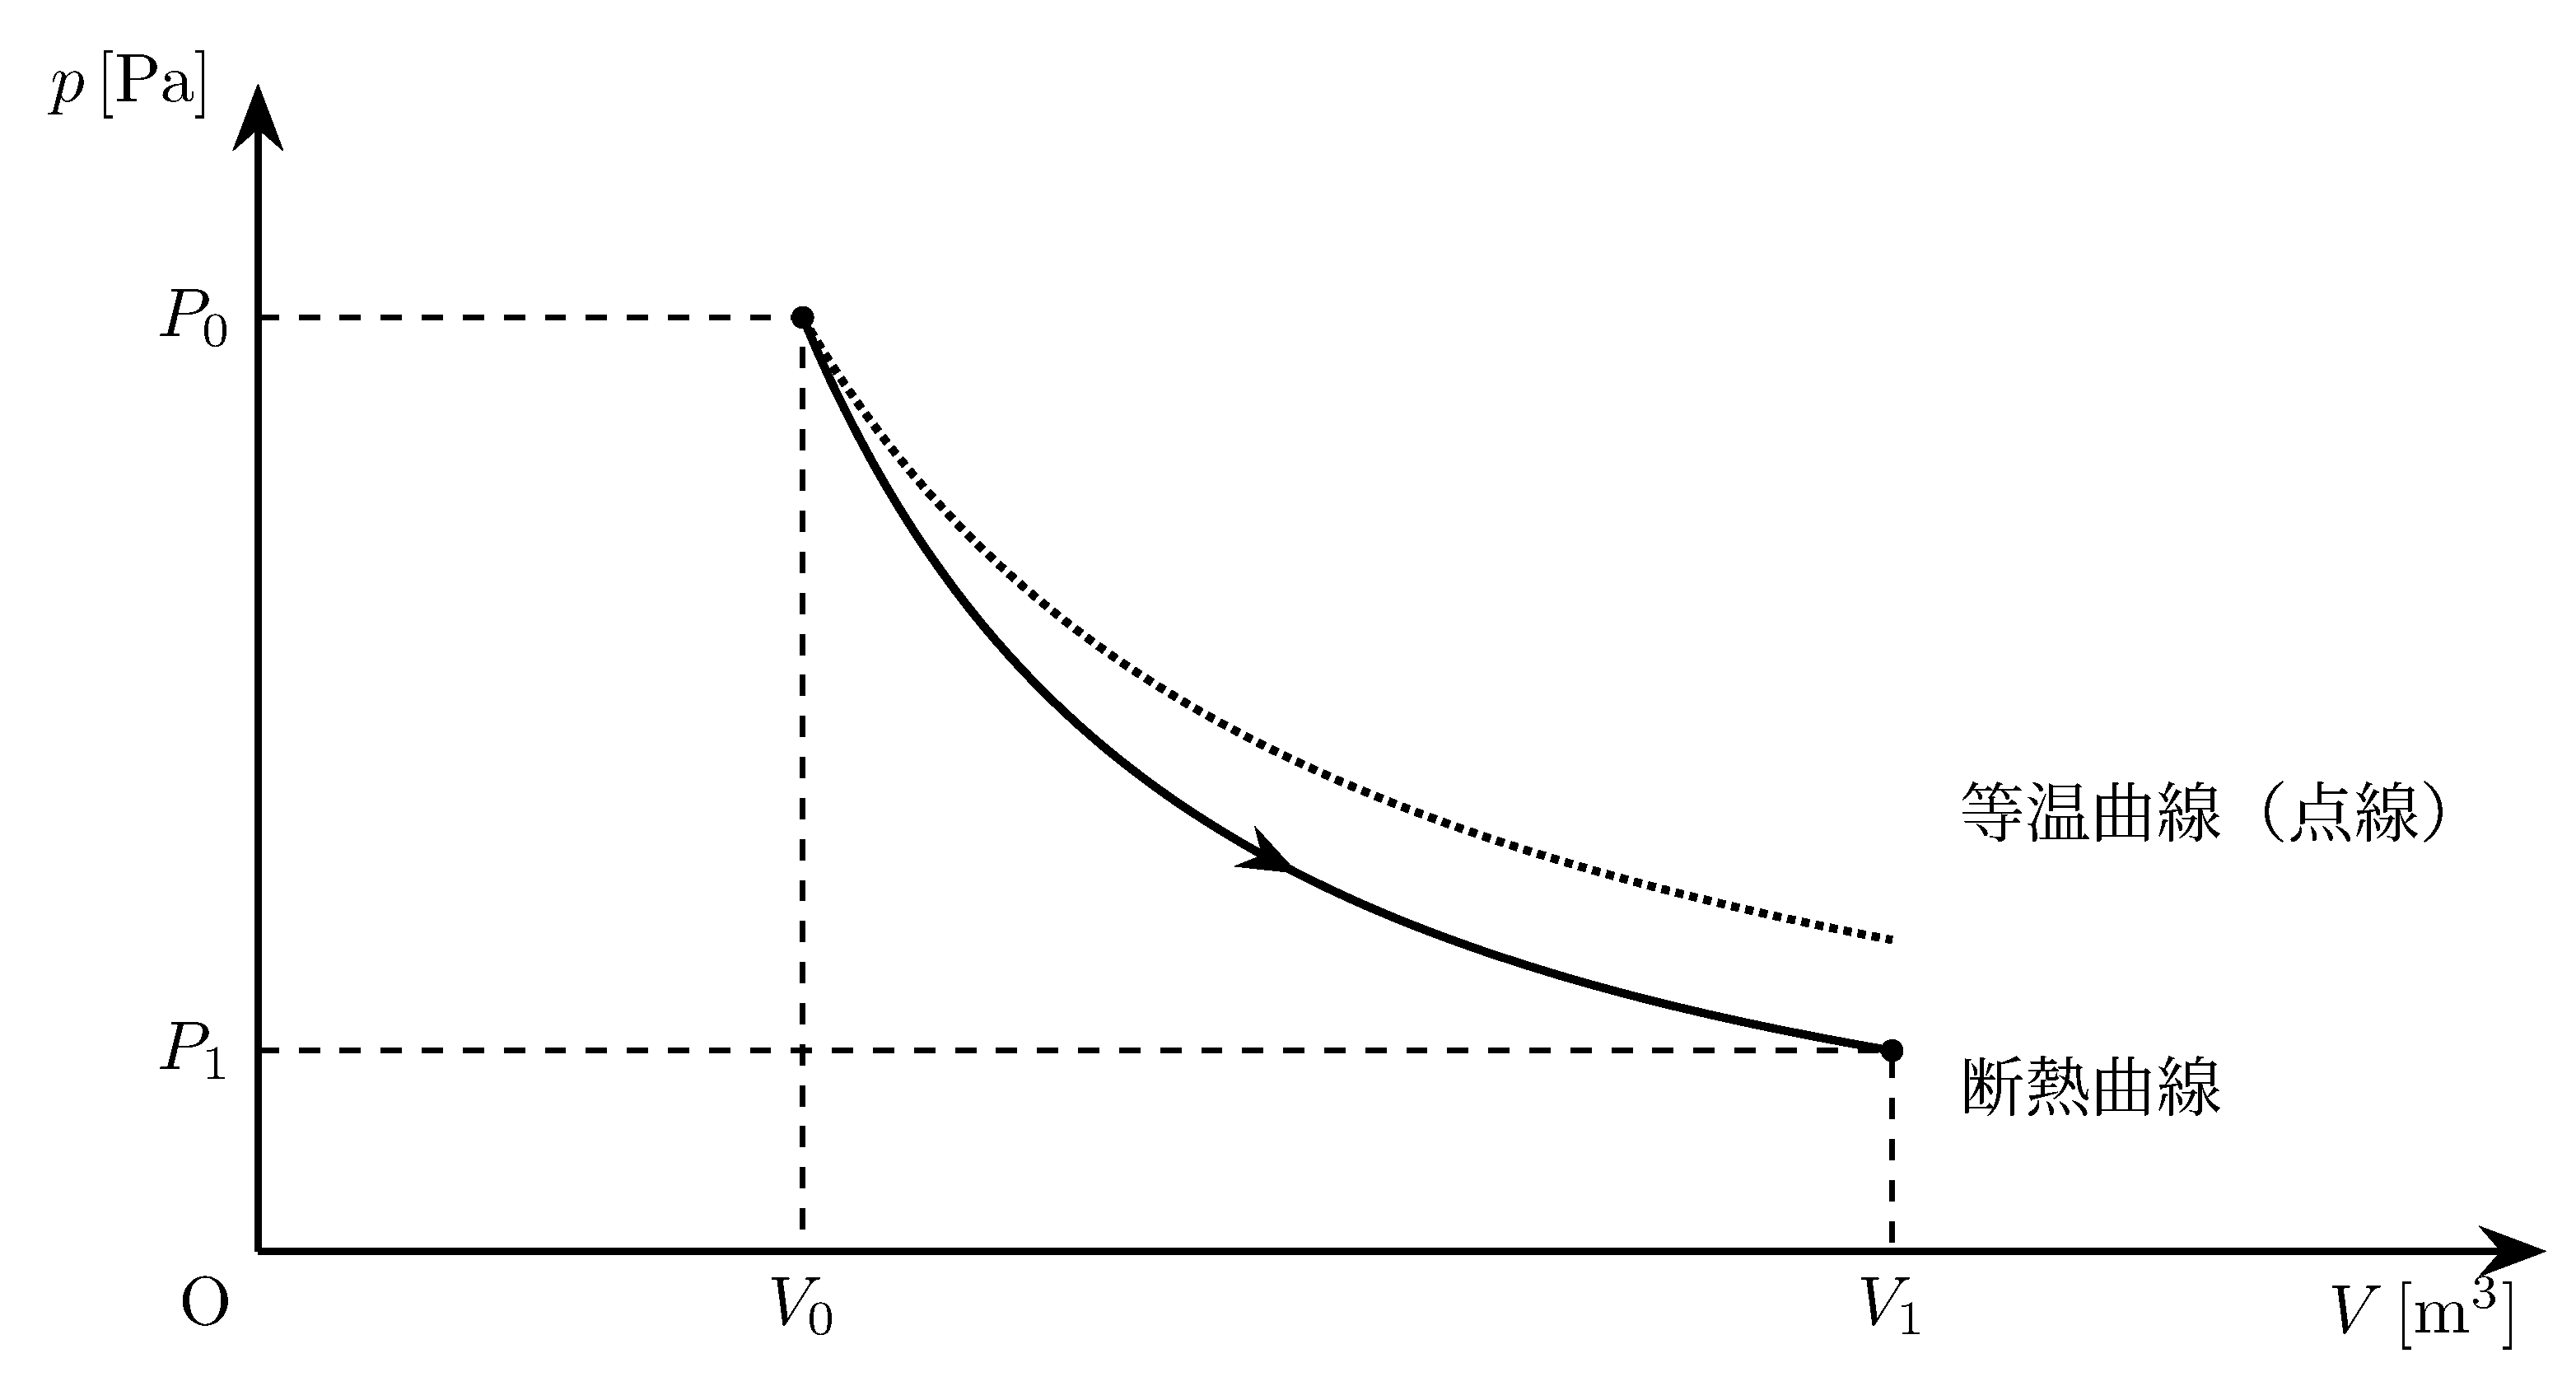
\includegraphics[keepaspectratio,width=106mm]{fig/ch17_ex13_pv.png}
       \fi
       \end{center}
       \hspace*{\fill}\Ans
\ko{3} 内部エネルギーは絶対温度だけで決まるので，
       \Ana{\Delta U=nC_V(T_1-T_0)\U{J}\Ans}
       $T_1<T_0$であるから$\Delta U<0$，すなわち内部エネルギーは減少する．
\ko{4} 断熱変化であるから$Q=0$であり，熱力学第一法則$\Delta U=Q+(-w)$より，
       \Ana{w=-\Delta U=nC_V(T_0-T_1)\U{J}\Ans}
\ko{5} マイヤーの関係式$C_P=C_V+R$より$\gamma-1=\dfrac{C_P}{C_V}-1=\dfrac{R}{C_V}$である．ポアソンの式\mbox{$TV^{\gamma-1}=（一定）$}を始状態と終状態に適用して，
       \Ana{T_0V_0^{\gamma-1}=T_1V_1^{\gamma-1}}
       これを$V_1$について解くと，
       \Ana{V_1=V_0\left(\frac{T_0}{T_1}\right)^{\frac{1}{\gamma-1}}
             =V_0\left(\frac{T_0}{T_1}\right)^{\frac{C_V}{R}}\U{m^3}\Ans}
       $T_0>T_1$であるから$V_1>V_0$となり，膨張していることが確かめられる．
\end{komon}
\end{kaitou}
\end{reidaiunit}

%%%%%%%%%%%%%%%%%%%%  例題14（17.3 のまとめ枠の直後）  %%%%%%%%%%%%%%%%%%%%
\begin{reidaiunit}
\begin{reidai}{断熱自由膨張}
\begin{zuright}{52mm}
\hspace{1zw}断熱材で作られた容器の中に，仕切板を隔てて図の左側の空間にのみ定積モル比熱が$C_V\U{J/mol\cdot K}$，温度が$T_0\U{K}$の理想気体が$n\U{mol}$封入されている．
\zusep
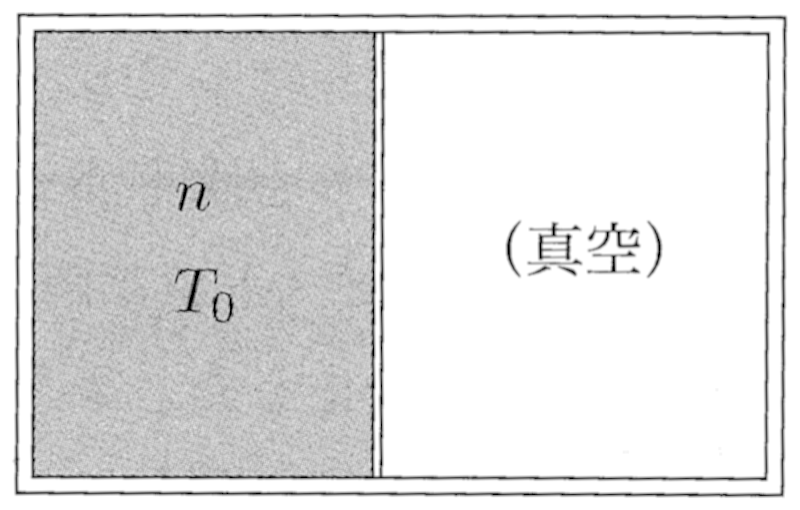
\includegraphics[keepaspectratio,width=52mm]{fig/ch17_ex14_box1.png}
\end{zuright}
\begin{komon}
\ko{1} この仕切板に穴を開けると気体は右側へと拡散していく．十分時間がたったのちの気体の温度$T^\prime\U{K}$を求めよ．
\end{komon}
\begin{zuright}{52mm}
\hspace{1zw}先と同じく断熱材で作られた容器の中に，仕切板を隔てて図のように左側，右側それぞれに異なる気体を封入する．左側（体積$V_1\U{m^3}$）には定積モル比熱$C_{V1}\U{J/mol\cdot K}$，温度が$T_1\U{K}$の理想気体が$n_1\U{mol}$だけ封入されており，右側（体積$V_2\U{m^3}$）には定積モル比熱$C_{V2}\U{J/mol\cdot K}$，温度が$T_2\U{K}$の理想気体が$n_2\U{mol}$だけ封入されている．
\zusep
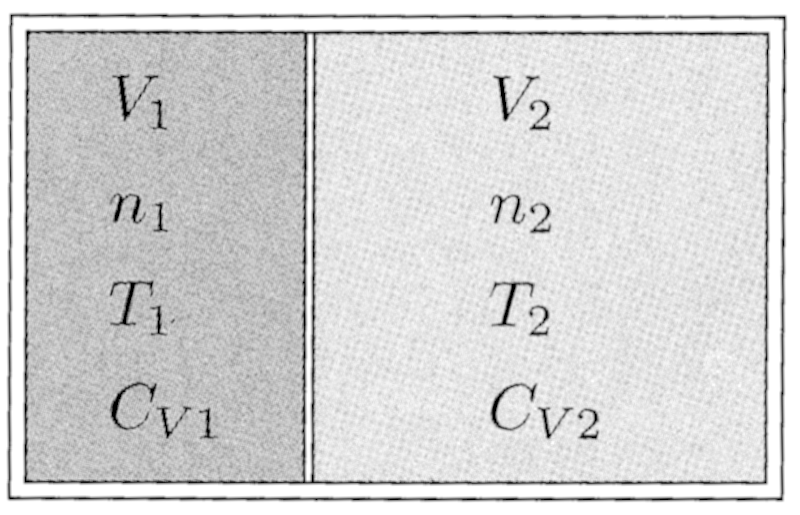
\includegraphics[keepaspectratio,width=52mm]{fig/ch17_ex14_box2.png}
\end{zuright}
\begin{komon}
\ko{2} この仕切板を取り外し，外界との熱のやり取りを断って2つの気体を混合する．十分時間がたったのちの温度$T\U{K}$を求めよ．
\end{komon}
\end{reidai}

\begin{sisinE}
どちらも{\gtfamily 容器全体を一つの系とみなして熱力学第一法則を立てる}．容器の体積は変わらないので外界と仕事のやり取りはなく（$W=0$），断熱材で作られているので熱のやり取りもない（$Q=0$）．したがって容器全体の内部エネルギーの変化は$\Delta U=0$である．

(2)では，容器全体の内部エネルギー変化は左側の気体の変化と右側の気体の変化の和であることを使う．
\end{sisinE}

\Key{真空中への断熱自由膨張 $\Rightarrow$ 箱全体に対しての熱力学第一法則}

\begin{kaitou}
\begin{komon}
\ko{1} 容器全体を一つの系とみなすと，体積が変わらないので$W=0$，断熱材なので$Q=0$である．よって熱力学第一法則より
       \Ana{\Delta U=Q+W=0}
       一方，内部エネルギーの変化は$\Delta U=nC_V(T^\prime-T_0)$と表せるから，$nC_V\neq 0$より$T^\prime-T_0=0$，すなわち
       \Ana{T^\prime=T_0\U{K}\Ans}
\ko{2} こちらも容器全体では$Q=0$, $W=0$であるから$\Delta U=0$である．混合後の温度を$T\U{K}$とすると，左側の気体の内部エネルギー変化と右側の気体の内部エネルギー変化の和が$\Delta U$であるから，
       \Ana{n_1C_{V1}(T-T_1)+n_2C_{V2}(T-T_2)=0}
       これを$T$について解いて，
       \Ana{T=\frac{n_1C_{V1}T_1+n_2C_{V2}T_2}{n_1C_{V1}+n_2C_{V2}}\U{K}\Ans}
\end{komon}
\end{kaitou}
\end{reidaiunit}
